\documentclass[../../thesis.tex]{subfiles}

\begin{document}

Our work in this thesis can be seen as a tangent of the paper "Vector Quantized Time Series Generation with a Bidirectional Prior Model" \cite{TimeVQVAE}. 
We simplify the model architecture by omitting the high-low frequency split, which reduces the model to what they refer to as "naive TimeVQVAE" in their paper. We expand on naive TimeVQVAE  with a self-supervised extension.\newline

The overarching objective in creating our model is to learn more expressive latent representations for better time series generation. We want to improve the reconstruction capabilities of the tokenization model. The rationality is that if the tokenization model reconstructs well the latent representations contains all relevant information of the input. We simultaneously want enforce better class separability in the latent representations, as we hypothesize that such additional structure eases learning of the generative model, both unconditional and conditional generation.\newline

To improve on the reconstruction we add a regularizing term by reconstructing augmented views. We hypothesize that the model generalizes better to unseen data by letting the decoder "see" the augmented views.\newline
To separate classes better we introduce a non contrastive self supervised loss. The intuition being that the representation of original and augmented views are pushed closer together by the SSL loss. We further enforce this hypothesis by using augmentations that preserve the overall semantics of the class conditional distributions. \newline






\begin{figure}[h]
    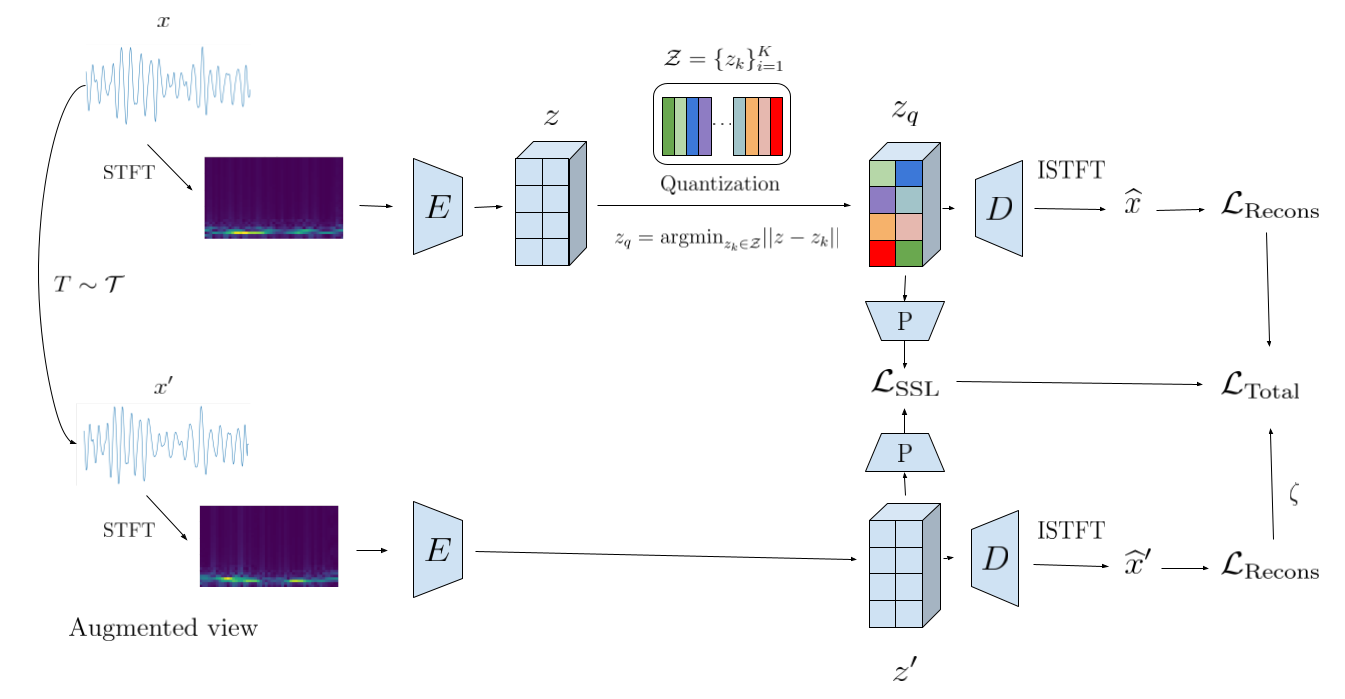
\includegraphics[scale=0.27]{Siam-VQVAE.png}
    \centering  
    \caption{Overview of proposed model.}
\end{figure}


\section{Stage 1: Tokenization}


\subsection{VQVAE}
The the naive VQVAE model as described in \cite{TimeVQVAE} is baseline for our experiments.\\

An encoder, decoder, and codebook are to be optimized by compressing the input into discrete latent space, minimizing information loss by comparing input to the output, which ideally are equal. We follow \cite{TimeVQVAE} and augment time-series into time-frquency domain, but leave the high-low frequency split for future work.

\subsubsection{Method}
A schematic overview of the our VQ-VAE model is presented in "Figure here"\newline

A time series is first augmented into time-frequency domain using the Short-time Fourier Transform (cite pytorch stft). Then it is encoded into the continuous latent space, and is discretized by the codebook via the argmin process. In the argmin process the continuous token is compared to every discrete token in the codebook, and replaced by the closes discrete token in terms of euclidean distance. Then, the decoder maps the discrete token back to time-frequency domain, before finally being mapped back to time domain using the ISTFT.




\subsubsection{Implementation details}


\subsection{NC-VQ-VAE}
We have a common framework for the two SSL methods.\newline

As our overarching objective is to learn tokens that eases the prior learning and train a better generative model, we are primarily interested in lowering the reconstruction loss. This lead us to only provide augmented views to one branch. We denote the latent variables by $z$ and quantized latent variables $z_q$. All augmented values are denoted by as asterix, i.e $z'$ is a latent variable in the augmented branch.\newline

The framework is a siamese architecture with upper/original branch identical to the VQ-VAE model presented above. The the lower/augmented branch is identical, except for a lack of quantization layer. \newline

We compute a SSL loss between projected values of $z_q$ and $z'$. \newline

We compute reconstruction losses $\mathcal{L}_{\text{Rec}}(\hat{x})$ and $\mathcal{L}_{\text{Rec}}(\hat{x}')$, of both original and augmented view. 


\subsubsection{Method}

\subsubsection{Loss}


\subsubsection{Augmentations}
\TODO{Talk about soft vs hard augmentations. Temporal perserving vs not etc.}
We used the following collection of augmentation techniques.
\begin{itemize}
    \item Amplitude Resizing
    \item Window Warp
    \item Slice and Shuffle
    \item Gaussian noise
\end{itemize}

\subsubsection{Implementation details}

\subsection{Barlow Twins VQ-VAE}

\subsubsection{Model Architecture}


An encoder, decoder, codebook, and projector are to be optimized. Produce two augmented views of the time-series, augment views into time-frequency domain and encode into latent space. Choose one view for quantization, decoding and comparison to original time series (VQVAE loss). Project both latent embeddings and calculate Barlow loss. Update using both VQVAE and Barlow loss.

A schematic overview of the BT-VQ-VAE model is presented in "Figure here"



\subsection{VIbCReg VQ-VAE}

\subsubsection{Method}

\subsubsection{Implementation details}

\subsubsection{Training}

\section{Stage 2: Prior Learning}

\subsection{MaskGIT}
Regular MaskGIT, token context MaskGIT, learnable codebook MaskGIT


\section{UCR Archive}

\end{document}